\lipsum[1]

\section{Uma seção do apêndice}

\lipsum[2]

	\begin{figure}
		\centering
		
		\null\hfill
		\subfigure[Legenda curta][Legenda dessa figura]{
			\label{fig:figA}
			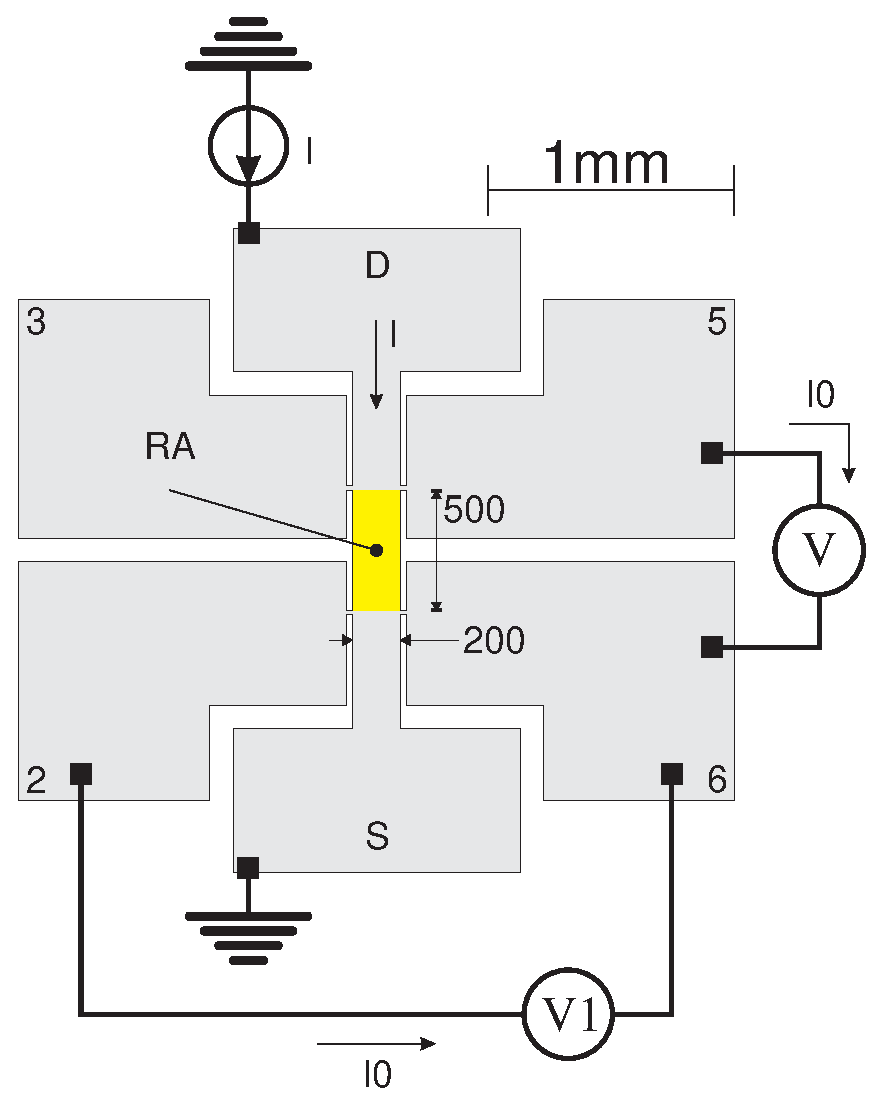
\includegraphics[width=0.4\textwidth]{bH}}%
		\hfill
		\subfigure[Legenda curta][Legenda dessa figura]{
			\label{fig:figB}
			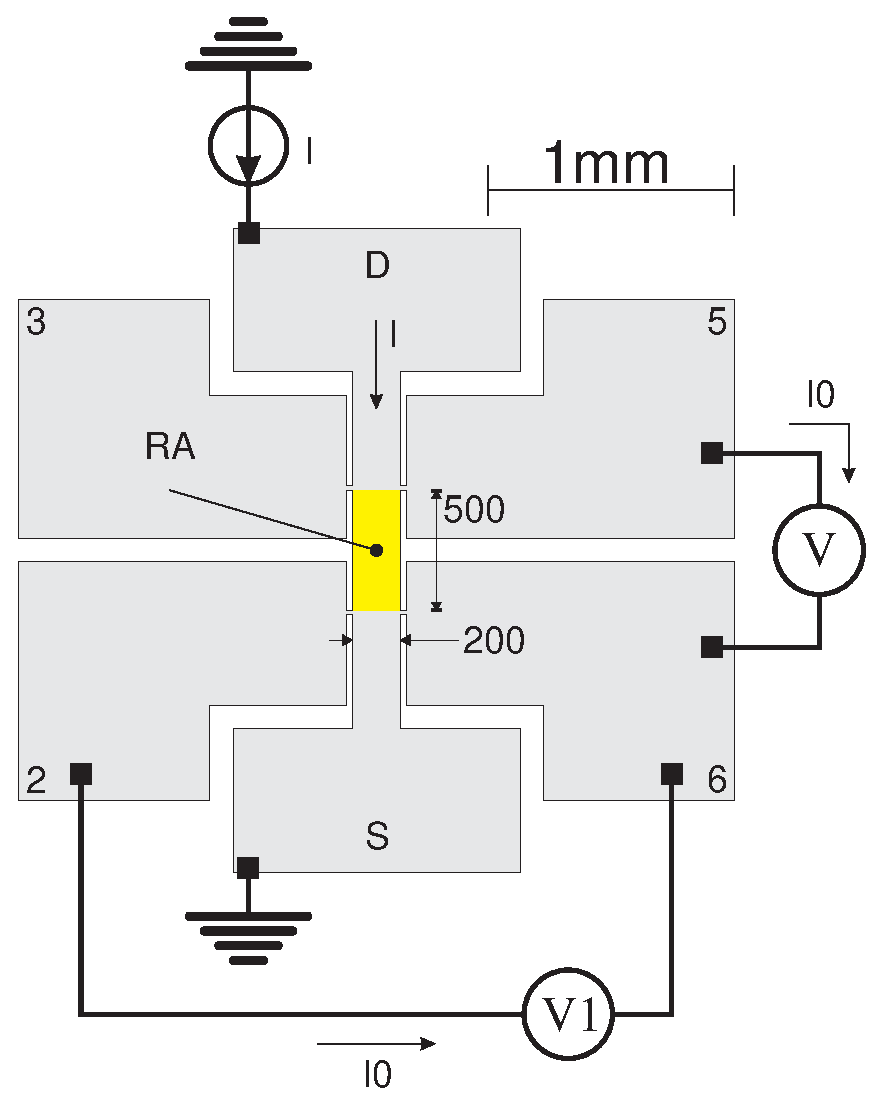
\includegraphics[width=0.4\textwidth]{bH}}%
		\hfill\null
		
		\caption[Legenda curta]{Legenda comum às duas figuras. A versão curta das legendas das duas figuras acima só aparecerão na lista de figuras se você definir o contador \ctr{lofdepth} (profundidade da lista de figuras) igual a 2.}
		\label{fig:AB}
	\end{figure}
	
\lipsum[6-7]